% \iffalse
\let\negmedspace\undefined
\let\negthickspace\undefined
\documentclass[journal,12pt,twocolumn]{IEEEtran}
\usepackage{cite}
\usepackage{amsmath,amssymb,amsfonts,amsthm}
\usepackage{algorithmic}
\usepackage{graphicx}
\usepackage{textcomp}
\usepackage{xcolor}
\usepackage{txfonts}
\usepackage{listings}
\usepackage{enumitem}
\usepackage{mathtools}
\usepackage{gensymb}
\usepackage{comment}
\usepackage[breaklinks=true]{hyperref}
\usepackage{tkz-euclide}
\usepackage{listings}
\usepackage{gvv}
\def\inputGnumericTable{}
\usepackage[latin1]{inputenc}
\usepackage{color}
\usepackage{array}
\usepackage{longtable}
\usepackage{calc}
\usepackage{multirow}
\usepackage{hhline}
\usepackage{ifthen}
\usepackage{lscape}
\usepackage{float}

\newtheorem{theorem}{Theorem}[section]
\newtheorem{problem}{Problem}
\newtheorem{proposition}{Proposition}[section]
\newtheorem{lemma}{Lemma}[section]
\newtheorem{corollary}[theorem]{Corollary}
\newtheorem{example}{Example}[section]
\newtheorem{definition}[problem]{Definition}
\newcommand{\BEQA}{\begin{eqnarray}}
\newcommand{\EEQA}{\end{eqnarray}}
\newcommand{\define}{\stackrel{\triangle}{=}}
\theoremstyle{remark}
\newtheorem{rem}{Remark}
\begin{document}

\bibliographystyle{IEEEtran}
\vspace{3cm}

\title{ANALOG-11.14.21}
\author{EE23BTECH11006 - Ameen Aazam$^{*}$% <-this % stops a space
}
\maketitle
\newpage
\bigskip

\renewcommand{\thefigure}{\theenumi}
\renewcommand{\thetable}{\theenumi}


\vspace{3cm}
\textbf{Question :}
You are riding in an automobile of mass 3000 kg. Assuming that you are examining the oscillation characteristics of its suspension system. The suspension sags 15 cm when the entire automobile is placed on it. Also, the amplitude of oscillation decreases by 50\% during one complete oscillation. Estimate the values of
\begin{enumerate}[label=(\alph*)]
    \item The spring constant \( K \)
    \item The damping constant \( b \) for the spring and shock absorber system of one wheel, assuming that each wheel supports 750 kg.
\end{enumerate}

\textbf{Solution :}
\begin{itemize}
\item \textbf{Parameters:}
    \begin{table}[h]
\begin{tabular}{|l|l|l|}
\hline
\textbf{Parameter} & \textbf{Value(SI)} & \textbf{Description} \\ \hline
$x$          & & Spring extension  \\ \hline
$x_{0}$ & 0.15 & Initial spring extension \\ \hline
$x_{p}$ & & Particular solution to $x$ \\ \hline
$x_{n}$ & & Null solution to $x$ \\ \hline
$v$          & $dx/dt$ & Velocity          \\ \hline
$a$          & $d^2x/dt^2$ & Acceleration      \\ \hline
$g$          & 9.8 & Gravitational acc \\ \hline
$m$          & 750 & Mass              \\ \hline
$k$          & $mg/x_{0}$ & Spring constant   \\ \hline
$b$          &  & Damping constant  \\ \hline
$A_{0}$               & & Initial Amplitude  \\ \hline
$A$                   & & Amplitude  \\ \hline
$w$ & $\sqrt{\frac{k}{m}-\left(\frac{b}{2m}\right)^2}$ & Angular frequency \\ \hline
$\phi$ & & Initial phase \\ \hline
$T$ & $2\pi\sqrt{\frac{m}{k}}$ & Approximate time peiod \\ \hline
$A_{1}, A_{2},h,s$ & & Constants \\ \hline
$s_{1},s_{2}$ & & Values of $s$ \\ \hline
$F_{net}$ & & Net force acting on the mass \\ \hline
$F_{1}$ & & Spring force \\ \hline
$F_{2}$ & & Damping force\\ \hline
\end{tabular}
\end{table}




\item\textbf{Part-a:}
    Initially the automobile is in rest, so we can use,
    \begin{align}
&mg = kx \\
\Rightarrow &k=\frac{mg}{x}
    \end{align}

\item \textbf{Part-b:}
\begin{figure}[h]
        \centering
        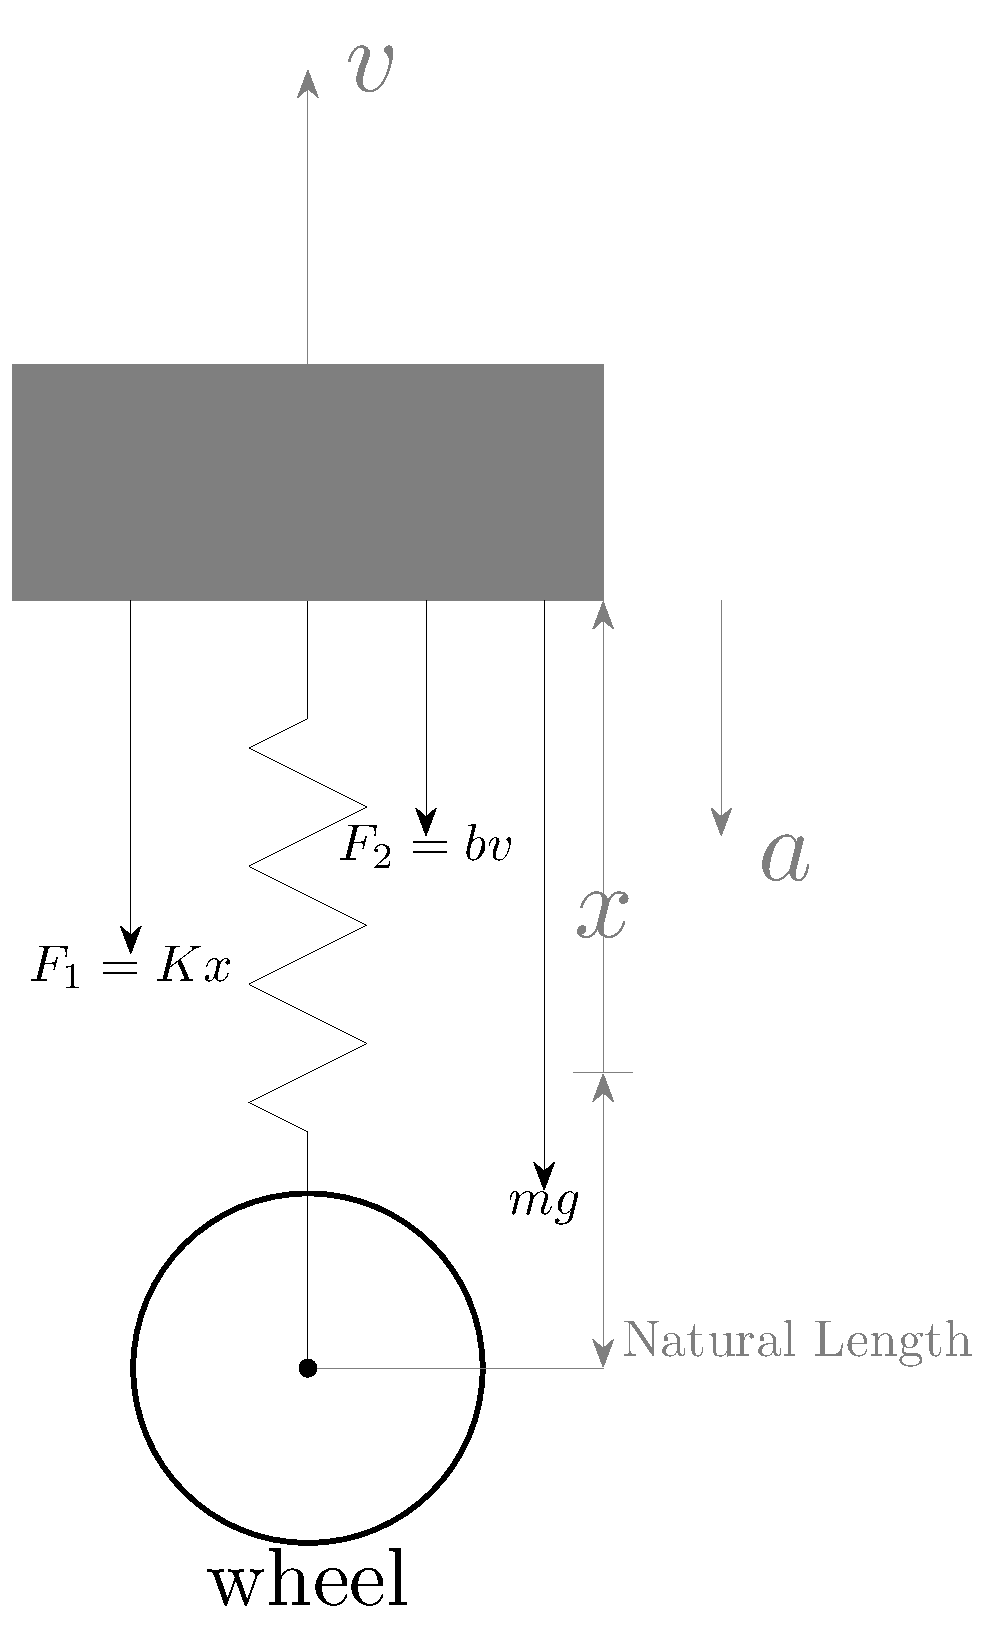
\includegraphics[width=0.8\linewidth]{11_14_21_fbd.pdf}
        \caption{FBD of the damped oscillation system}
        \label{fig:enter-label}
    \end{figure}

Now, as the oscillation begins we would have the force equation from the FBD as,
\begin{align}
    &F_{net}=F_{1}+F_{2}+mg\\
    \Rightarrow &F_{net}=Kx+bv+mg\\
    \Rightarrow &ma=kx+bv+mg\\
    \Rightarrow &-m\frac{d^2x}{dt^2}=kx+b\frac{dx}{dt}+mg\\
    \Rightarrow &\frac{d^2x}{dt^2}+\left(\frac{b}{m}\right)\frac{dx}{dt}+\left(\frac{k}{m}\right)x=-g
\end{align}
So, $x$ can be written as,
\begin{align}
x=x_{p}+x_{n}
\end{align}
And a constant input implies a constant $x_{p}$.
Putting $x_{p}$ in (7) we get,\\
\begin{align}
x_{p}=-\frac{mg}{k}
\end{align}
And for $x_{n}$ consider the equation,\\
\begin{align}
\frac{d^2x}{dt^2}+\left(\frac{b}{m}\right)\frac{dx}{dt}+\left(\frac{k}{m}\right)x=0
\end{align}
$x_{n}$ will be of the form,
\[x_{n}=he^{st}\]
using this in (11) we get,
\begin{align}
    &s^2+\left(\frac{b}{m}\right)s+\left(\frac{k}{m}\right)=0 \\
    \Rightarrow &s_{1}=-\frac{b}{2m}+\sqrt{\left(\frac{b}{2m}\right)^2-\frac{k}{m}} \\
    &=-\frac{b}{2m}+jw \\
    \Rightarrow &s_{2}=-\frac{b}{2m}-\sqrt{\left(\frac{b}{2m}\right)^2-\frac{k}{m}} \\
    &=-\frac{b}{2m}+jw
\end{align}
So we have $x$ as,
\begin{align}
    &x=A_{1}e^{s_{1}t}+A_{2}e^{s_{2}t}-\frac{mg}{k} \\
    &=A_{1}e^{\left(-\frac{b}{2m}+jw\right)t}+A_{2}e^{\left(-\frac{b}{2m}-jw\right)t}-\frac{mg}{k} \\
    &=e^{-\frac{b}{2m}t}\left(A_{1}e^{jwt}+A_{2}e^{-jwt}\right)-\frac{mg}{k} \\
    &=e^{-\frac{b}{2m}t}\left[(A_{1}+A_{2})\cos{wt}+(A_{1}-A_{2})j\sin{wt}\right]-\frac{mg}{k} \\
    &=A_{0}e^{-\frac{b}{2m}t}\sin{(wt+\phi)}-\frac{mg}{k}
\end{align}
From (20) we have the amplitudue \text{A},
\begin{align}
    &A=A_{0}e^{-\frac{b}{2m}t} \\
    \Rightarrow &\frac{A_{0}}{2}=A_{0}e^{-\frac{b}{2m}T} \\
    \Rightarrow &e^{\frac{b}{2m}T}=2 \\
    \Rightarrow &\frac{b}{2m}2\pi\sqrt{\frac{m}{k}}=\ln{2} \\
    \Rightarrow &b=\frac{\sqrt{mk}\ln{2}}{\pi}
\end{align}
\textbf{Answer :}
Now substituting the values of the parameters  we have \\
\item \textbf{Part-a:} The spring constant, $k=4.9\times10^4 \text{N/m}$.
\item \textbf{Pat-b:} The damping constant, $b=1337.53 \text{Kg/s}$.
\end{itemize}

\end{document}


